\selectlanguage{english}
\chapter{The CMS detector at LHC}
\label{Chapter2}
%SourceDoc tesi.tex

\section{The Large Hadron Collider}
Approved in the early '90s and started up in the 2008, the \textit{Large Hadron Collider} is currently the world's largest and most powerful particle accelerator. \\
Its main purpose is to help in testing the predictions of different theories of particle physics, including the search of the Higgs boson and the dark matter. \\
Built at a mean depth of 100m, beneath France-Switzerland border near Geneva, in the tunnel formerly used to house the Large Electron-Positron collider (LEP), the LHC  of a 26.7km ring of superconducting magnets with a number of accelerating structures to boost the energy of the particles along the way. It is not a perfect circle: it is made of eight arcs and eight 'insertions'. The arcs are long 106.9m with a curvature of 2.84km containing 1232 superconductive dipoles. The LHC dipoles use Niobium-Titanium (NbTi) cables at a temperature of 1.9K, pumping superfluid helium into the magnet system, where they become superconducting; a current of 11850A flows in the dipoles to create the high magnetic field of 8.33 T required to bend the beams around the ring. 
%due to geological consideration, it has a slight gradient of 1.4\% and its depth varies between 150m (under the Jura) and 50m (towards lake Geneva ). 
The insertions instead consist of a long straight section of 528m plus two (one at each end) transition regions. They contains the radiofrequency cavities to increase beam energy (0.5 MeV per period): there are eight cavities per beam, each delivering 2MV (an accelerating field of 5MV/m) at 400MHz operating at 4.5K. Particular kind of insertion are quadrupoles, special magnets used to focus the beam down to the smallest possible size at the collision points: there 392 quadrupoles in LHC. \\
In the LHC each particle beam is accelerated up to 6.5 TeV (7 TeV is the designed energy not yet reached) but it is the last element of the accelerating chain. \\
The proton beam is created by using an electric field to pull the electrons from hydrogen atoms and start the acceleration. Protons are injected into the PS Booster (PSB) at an  energy of 50 MeV from Linac2 (Linear Accelerator 2). The booster comprises four superposed rings: this is because at low energy intensity, the quality of the beams suffers from the repulsive forces between particles. By splitting up the injected beam this effect gets reduced. Once the beam reaches the energy of 1.4 GeV it is extracted and injected into Proton Synchrotron (PS). With a circumference of 628 m, the PS accelerates the beams up to 26 GeV when they are extracted and sent to the Super Proton Synchrotron (SPS). Built in the '70, the SPS has a length of 7 km. The beam is injected at 26 GeV, ramped up to 450 GeV and extracted to the LHC. At the SPS, the boson W and Z were discovered and this led Rubbia and Simon van der Meer to win the Nobel prize. In \figurename~\ref{Cern-Accelerator-Complex}  a complete scheme of the accelerator chain of the LHC.\\
\begin{figure}[htbp]
\centering
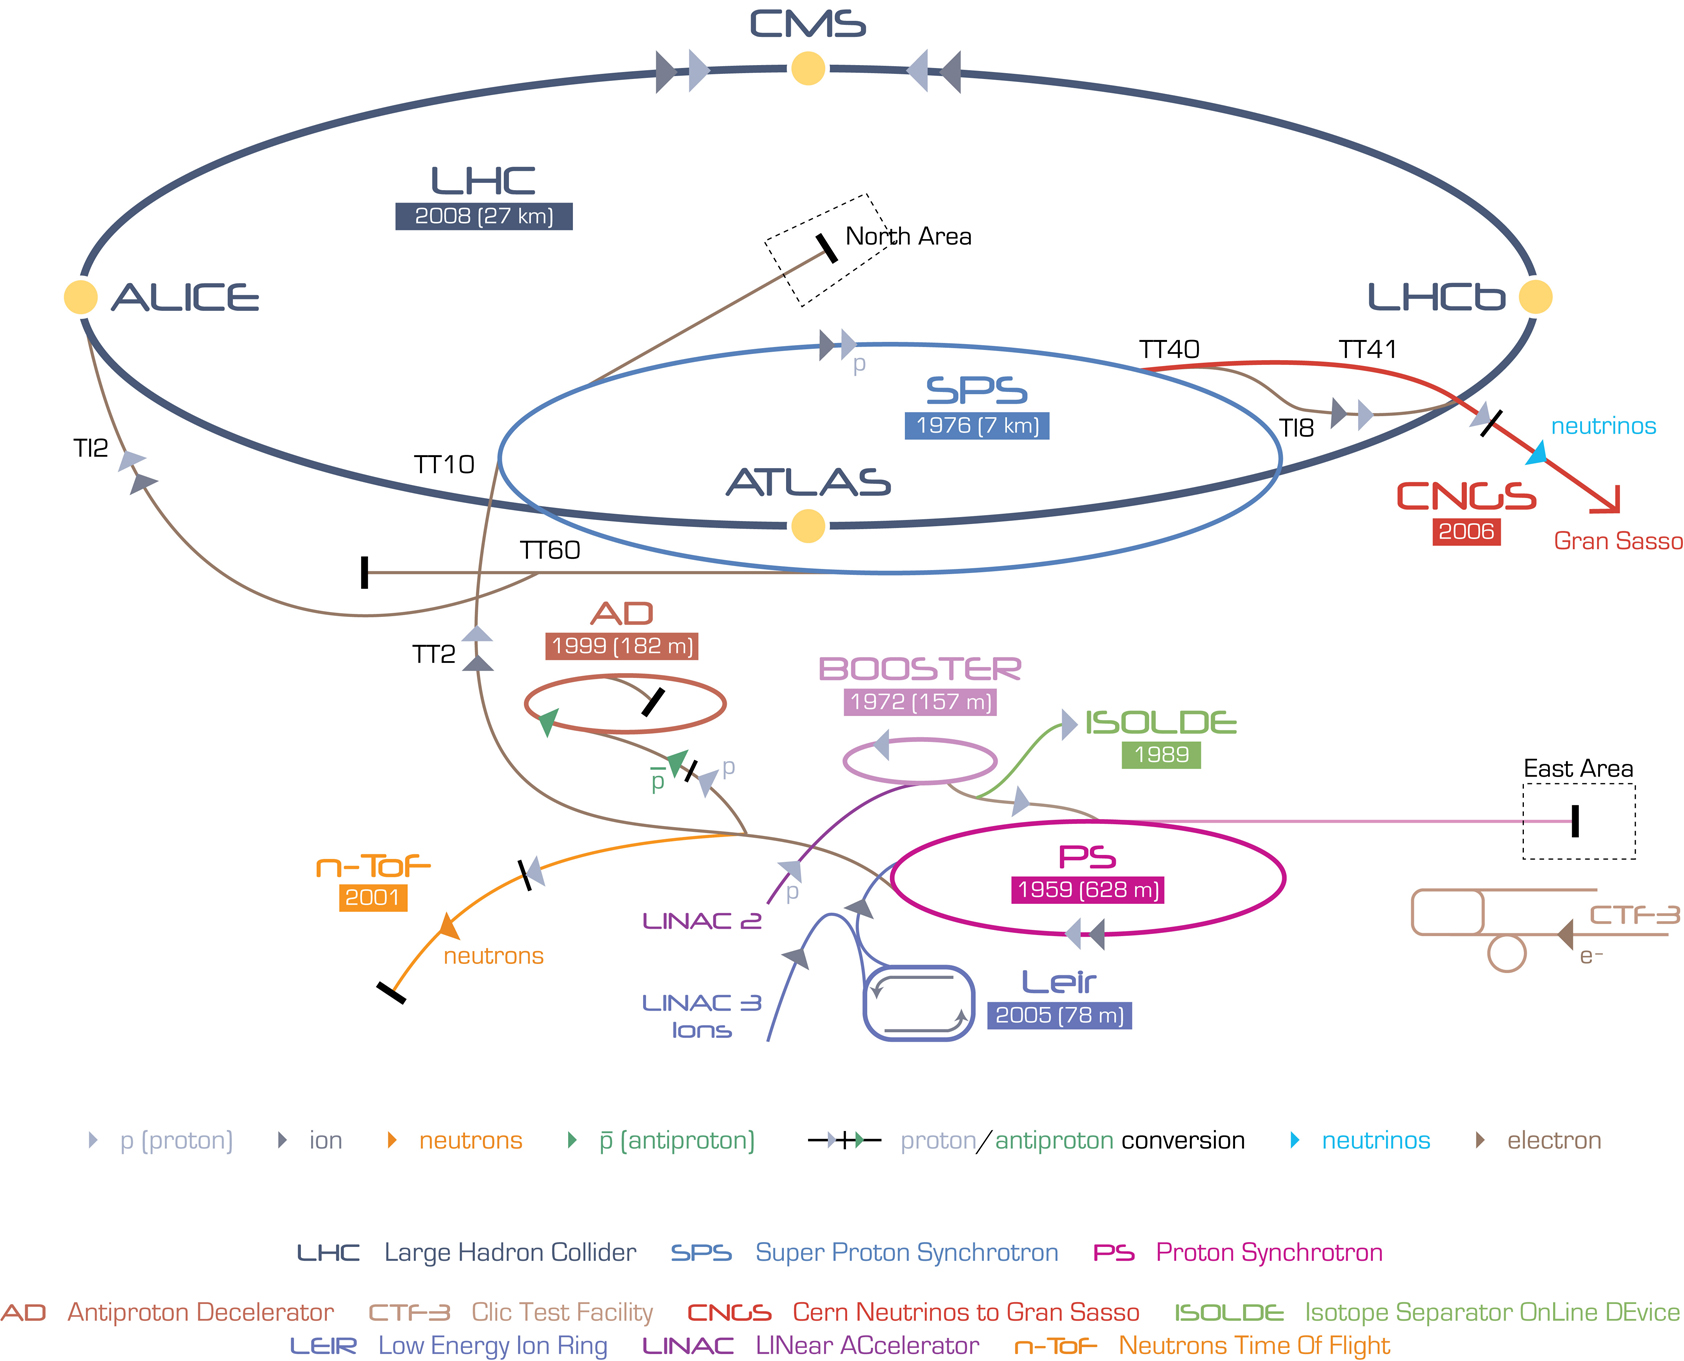
\includegraphics[width=0.65\textwidth]{Images/Cern-Accelerator-Complex}
\caption{Accelerator scheme at CERN.}
\label{Cern-Accelerator-Complex}
\end{figure}
Once the energy-working point is reached, the beams are made to collide at four locations around the LHC, corresponding to the position of four particles detectors: ALICE (\emph{A Large Ion Collider Experiment}), ATLAS (\emph{A Toroidal LHC ApparatuS}), CMS (\emph{Compact Muon Solenoid}) and LHCb (\emph{Large Hadron Collider beauty}). In addition to these, there are other three experiment installed at the LHC: TOTEM (\textit{TOTal Elastic and diffractive cross section Measurement}) installed close to CMS, MoEDAL (\textit{Monopole and Exotics Detector at the LHC}) close to LHCb and LHCf (\textit{Large Hadron Collider forward}) near ATLAS. \\
The beams at LHC have a bunch structure as a direct consequence of the radio frequency acceleration scheme. Protons can only be accelerated when the RF field has the correct orientation when particles pass through an accelerating cavity. Under nominal operating conditions, each proton beam has 2808 bunches, with each bunch containing about $10^{11}$ protons. The bunch size is not constant around the ring getting squeezed as much as possibile around the interaction points in order to increase the probability of collision. They measure a few centimetres long and a millimetre wide when they are far from a collision point; as the bunches approach  the collision points, they are squeezed to about $20\ \mu m$. LHC uses a bunch spacing of 25 ns (or 7.5 m) corresponding to a frequency of 40 MHz. \\
High frequency and small beam section, let to increase the number of events, the so call \textit{rate}, defined as:
\begin{equation}
\mathcal{R} = \sigma \times \mathcal{L}
\label{rate}
\end{equation}
In \ref{rate}, $\sigma$ represents the cross section of a particular event and $\mathcal{L}$ is the luminosity:
\begin{equation}
\mathcal{L} = \frac{f k_{B} N^{2}_{P}}{4 \pi \sigma_{x} \sigma_{y}}
\label{luminosity}
\end{equation}
where f is the frequency, $k_{B}$ the number of bunch and $N_{P}$ the number of proton in each bunch, $\sigma_{x}$ and $\sigma_{y}$ instead are the transversal sizes of the bunch at interaction point. \\
In \tablename~\ref{LHC_parameteres} are reported the designed LHC parameters and the ones reached at the end of RunII in 2018.
\begin{table}[htbp]	
	\begin{center}
		\begin{tabular}{p{6cm}*{3}{c}}
			\hline   &  & Design & 2018  \\
			\hline
			\hline
			\bfseries Centre of mass energy & \emph{E} & 14 TeV & 13 TeV \\
			\hline
			\bfseries Luminosity & \emph{L} & 10$^{34}$ cm$^{-2}$s$^{-1}$ & --- \\
			\hline
			\bfseries Time spacing &  & 25 ns & 25 ns\\
			\hline
			\bfseries Num. of bunches& \emph{k$_{B}$} & 2808 & ---\\
			\hline
			\bfseries Num. protons per bunch & \emph{N$_{p}$} & 1.15$\times$10$^{11}$ & ---\\
			\hline
			\hline
		\end{tabular}
	\end{center}
	\caption{LHC parameters}
	\label{LHC_parameteres}
\end{table}

\section{The Compact Muon Solenoid}
CMS, \textit{Compact Muon Solenoid}, is one of the four biggest experiment installed at LHC: it is a general-purpose detector designed to cover the widest possible range of physics at LHC, from precision measurements of the Higgs boson to searches for new physics beyond the Standard Model \cite{CMS_Detector}. \\
In order to manage with these goals,  the detector requirements for CMS can be summarised as follows: 
\begin{itemize}
\item{Good muon identification and momentum resolution over a wide range of momenta in the region $|\eta|<2.5$, good dimuon mass resolution ($\approx 1\%$  at 100 GeV), and the ability to determine unambiguously the charge of muons with p < 1 TeV.}
\item{Good charged particle momentum resolution and reconstruction efficiency in the inner tracker. Efficient triggering and offline tagging of the $\tau$'s and b-jets, requiring pixel detectors close to the interaction region.}
\item{Good electromagnetic energy resolution, good diphoton and dielectron mass resolution ($\approx 1\%$  at 100 GeV), wide geometric coverage ($|\eta|<2.5$), measurement of the direction of the photons and correct localisation of the primary interaction vertex, $\pi^{0}$ rejection and efficienct photon and lepton isolation at high luminosity.}
\item{Good missing transverse energy and dijet mass resolution, requiring hadron calorimeters with a large hermetic geometric coverage ($|\eta|<5$) and with a fine lateral segmentation ($\Delta \eta \times \Delta \phi < 0.1\times0.1$)}.
\end{itemize}
The coordinate system adopted by CMS has the origin centered at the nominal collision point inside the experiment, the y-axis pointing vertically upward, and the x-axis pointing radially inward toward the center of the LHC. Thus, the z-axis points along the beam direction toward the Jura mountains from LHC Point 5. The azimuthal angle $\phi$ is measured from the x-axis in the x-y plane and the radial coordinate in this plane is denoted by r. The polar angle $\theta$ is measured from the z-axis. Pseudorapidity is defined as $\eta = - \ln \tan(\theta /2)$. Thus, the momentum and energy transverse to the beam direction, denoted by $p_{T}$ and $E_{T}$ , respectively, are computed from the x and y components. The imbalance of energy measured in the transverse plane is denoted by $E_{T}^{miss}$. \\
The overall layout of CMS is shown in \figurename~\ref{CMS_Layout}. It is is a 21.6 m long cylinder with a diameter of 14.6 m and a total weight of 12500 tons. 
%Its main feature is the cylindrical coil of superconducting cable that generates a magnetic field of 4 T. 
%It Large bending power is needed to measure precisely the momentum of high-energy charged particles. \\
%In order to achieve good momentum resolution and alignment, a high magnetic field was chosen:
%The importance to have a huge magnetic field is linked with the necessity to measure as precise as can, the momentum of the particles:
%\begin{equation}
%p[TeV] = 0.3 \cdot B[T] \cdot R[km]
%\end{equation}
%with the relative error  $\sigma_{p}/p \propto 1/B$. \\
At its  center sits 13 m long and 5.9 m inner diameter, 4-T superconducting solenoid providing a large bending power (12 Tm); its return field is large enough to saturate 1.5 m of iron, allowing 4 muon stations to be integrated to ensure robustness and full geometric coverage. Each muon station consists of several layers of aluminium drift tube (DT) and resistive pate chambers (RPCs) in the barrel region and cathode strip chambers (CSCs) in the endcap region complemented by RPCs. Inside the magnet coil, the inner tracker and the calorimetry are accommodated. The tracking system is a cylinder of length 5.8 m and a diameter 2.6 m: it consists of 10 layers of silicon microstrip detector plus 3 layers of silicon pixel detectors placed close to the interaction region to improve the measurement of the impact parameter of charged particle tracks as well as the position of the secondary vertices. This configuration provides the required granularity and precision allowing to deal with high track multiplicities. The tracking system is enveloped by the electromagnetic calorimeter (ECAL), made of lead tungstate ($PbWO_{4}$) crystals with coverage in pseudorapidity up to $|\eta| < 3.0$; in front of the endcap ECAL a preshower system is installed for $\pi^{0}$ rejection. The ECAL is surrounded by a plastic scintillator sampling hadron calorimeter (HCAL) with coverage up to $|\eta| < 3.0$. This central calorimetry is complemented by a "tail-catcher" in the barrel region. Coverage up to a pseudorapidity of 5.0 is provaded by an iron/quartz-fibre calorimeter. The forward calorimeters ensure full geometric coverage for the measurement of the transverse energy in the event.
\begin{figure}[htbp]
\centering
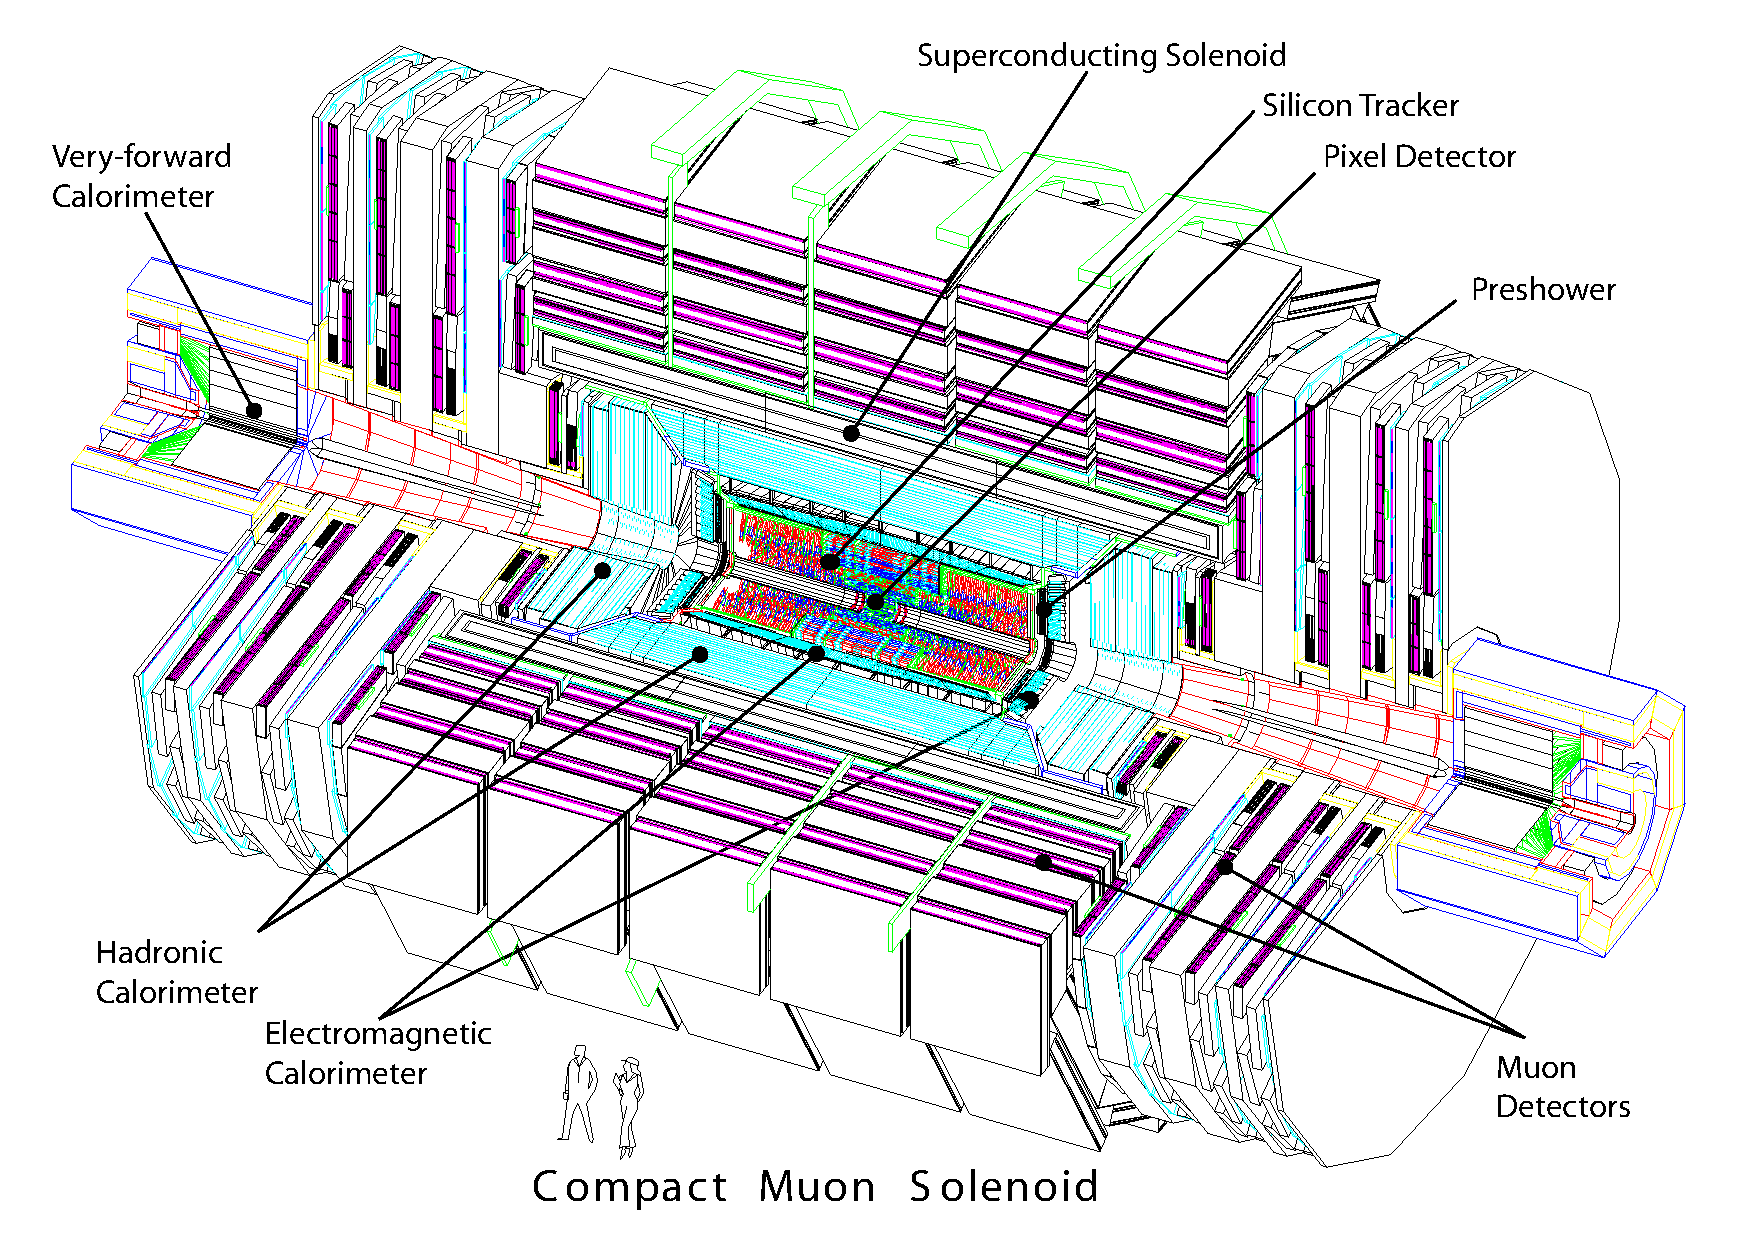
\includegraphics[width=0.7\textwidth]{Images/CMS_Layout.pdf}
\caption{CMS detector overview.}
\label{CMS_Layout}
\end{figure}

\subsection{The tracking system}
The tracking system of CMS \cite{Tracker_1, Tracker_2} is designed to provide a precise and efficient measurement of the trajectories of charged particles emerging from the LHC collisions, as well as a precise reconstruction of secondary vertices. It surrounds the interaction point and has a length of 5.8 m and a diameter of 2.5 m. The CMS solenoid provides a homogeneous magnetic field of 4 T over the full volume of the tracker. At the LHC design luminosity of $10^{34} cm^{-2} s^{-1}$ there will be on average about 1000 particles from more than 20 overlapping proton-proton interactions traversing the tracker for each bunch crossing, i.e. every 25 ns. Therefore a detector technology featuring high granularity and fast response is required, such that the trajectories can be identified reliably and attributed to the correct bunch crossing. \\
The CMS tracker is shown in \figurename~\ref{tracking_system}: it is composed of a pixel detector with three barrel layers at radii between 4.4 cm and 10.2 cm and a silicon strip tracker with 10 barrel detection layers extending outwards to a radius of 1.1 m. Each system is completed by endcaps which consist of 2 disks in the pixel detector and 3 plus 9 disks in the strip tracker on each side of the barrel, extending the acceptance of the tracker up to a pseudorapidity of $|\eta| < 2.5$.\\
\begin{figure}[htbp]
\centering
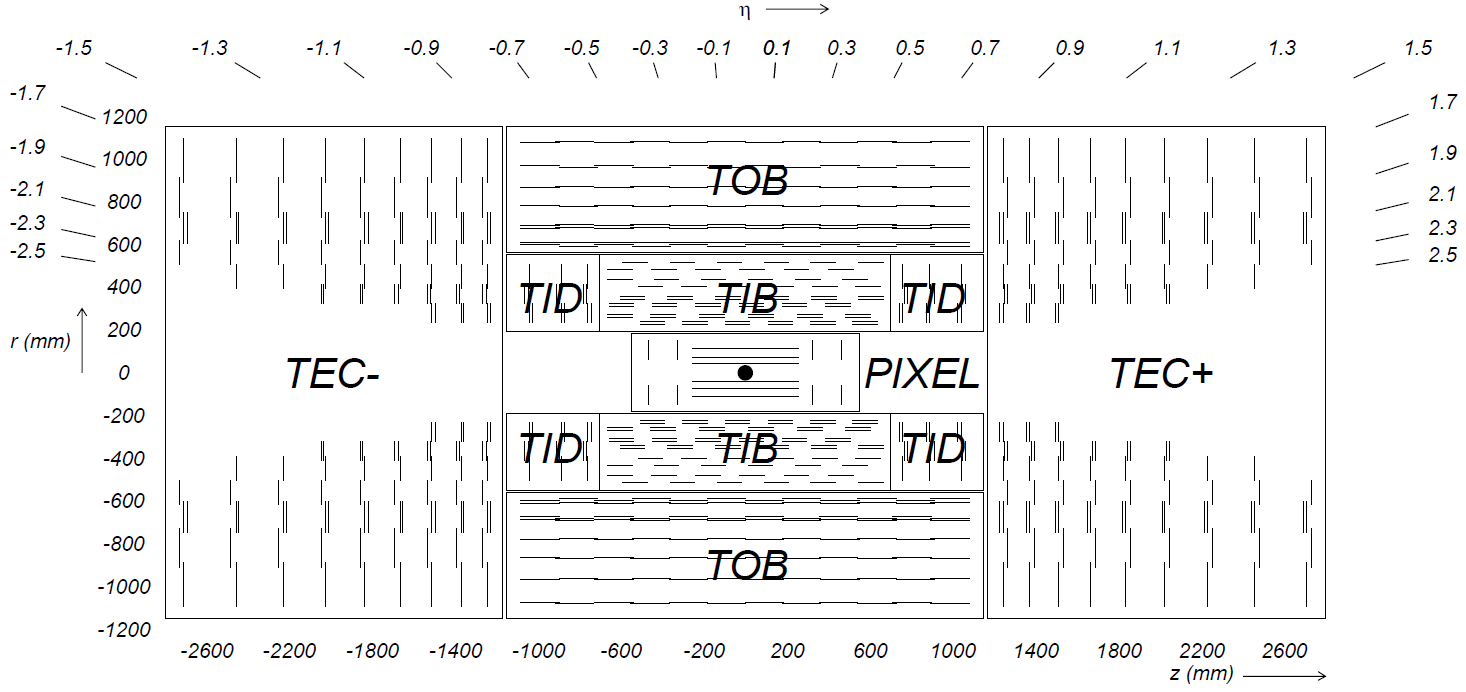
\includegraphics[width=0.7\textwidth]{Images/cmsTracker_TrackerLayout}
\caption{Schematic cross section through the CMS tracker in the $r-z$ plane: each line represents a detector module. Double lines indicate back-to-back modules which deliver stereo hits.}
\label{tracking_system}
\end{figure}
The tracker is the closest detector to the interaction point and it has a fundamental role in measuring kinematic variables of the particles. In \figurename~\ref{Tracker_performance} is shown the expected resolution of transverse momentum, transverse impact parameter and longitudinal impact parameter, as a function of pseudorapidity for single muons of transerve momentum of 1, 10 and 100 $GeV$. 
\begin{figure}[htbp]
\centering
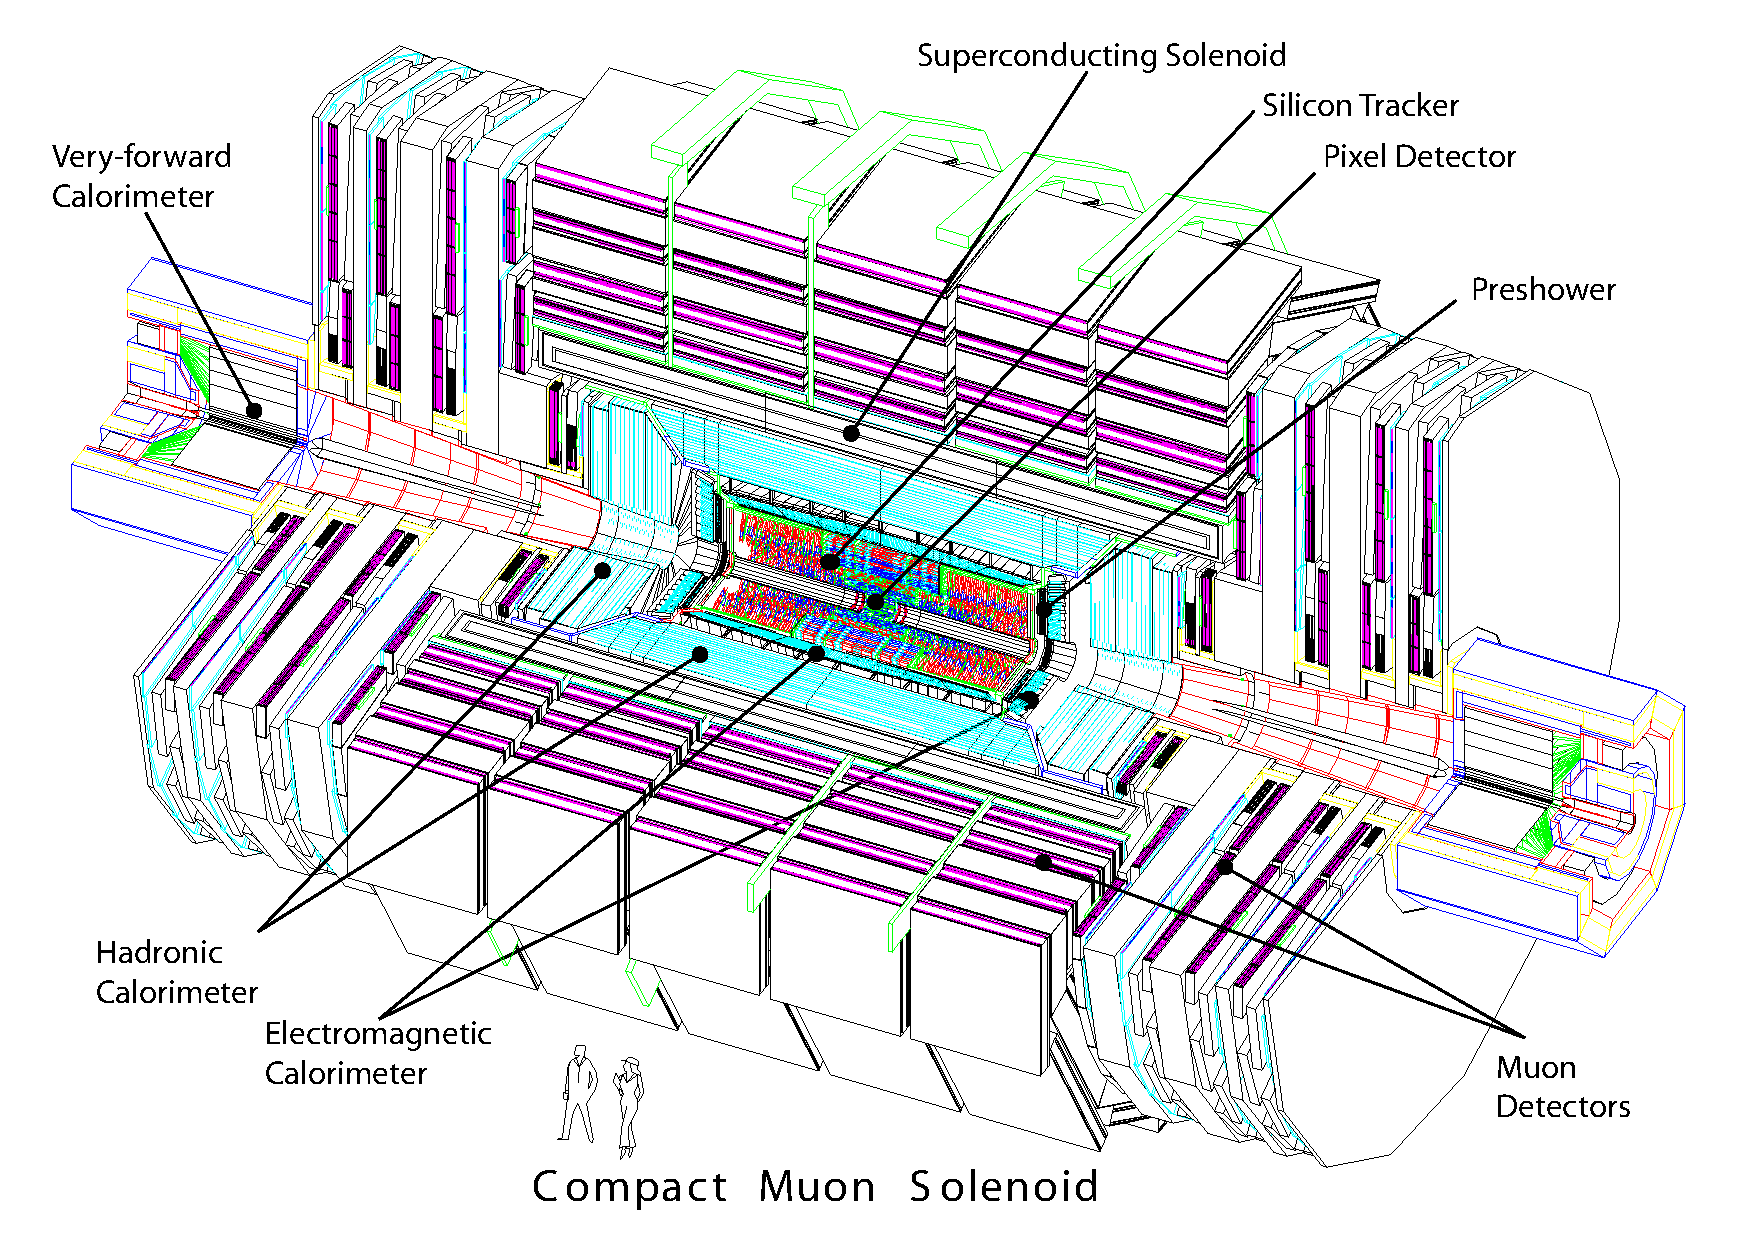
\includegraphics[width=0.1\textwidth]{Images/CMS_Layout.pdf}
\caption{Resolution for single muons with transverse momentum of 1, 10 and 100 GeV for several track parameters: transverse momentum (left panel), transverse impact parameter (middle panel), and longitudinal impact parameter (right panel).}
\label{Tracker_performance}
\end{figure}
For high momentum tracks (100 GeV) the transverse momentum resolution is around 1 - 2\% up to $|\eta| \approx 1.6$, beyond which it degrades due to the reduced lever arm. At a transverse momentum of 100 GeV multiple scattering in the tracker material accounts for 20 to 30\% of the transverse momentum resolution while at lower momentum it is dominated by multiple scattering. The transverse impact parameter resolution reaches 10 $\mu$m for high $p_{T}$ tracks, dominated by the resolution of the first pixel hit, while at lower momentum it is degraded by multiple scattering (similarly for the longitudinal impact parameter). \figurename~\ref{Tracker_performance}  shows the expected track reconstruction efficiency of the CMS tracker for single muons as a function of pseudorapidity: the efficiency is about 99\% over most of the acceptance and it decreases slightly at $|\eta| \approx 0$ due to gaps between the ladders of the pixel detector at z $\approx$ 0. At high $\eta$ the efficiency drop is mainly due to the reduced coverage by the pixel forward disks. \\ 
MATERIAL BUDGET
%Il tracker ricopre un?accettanza fino a |\eta| ? 2.5; `e spesso circa una lunghezza di radiazione e va da 0.4 X0 sulla verticale, crescendo fino a 1.8 X0 per |\eta| ? 1.4 e poi ridiscende ad una lunghezza per |\eta| ? 2.5.



\begin{figure}[htbp]
\centering
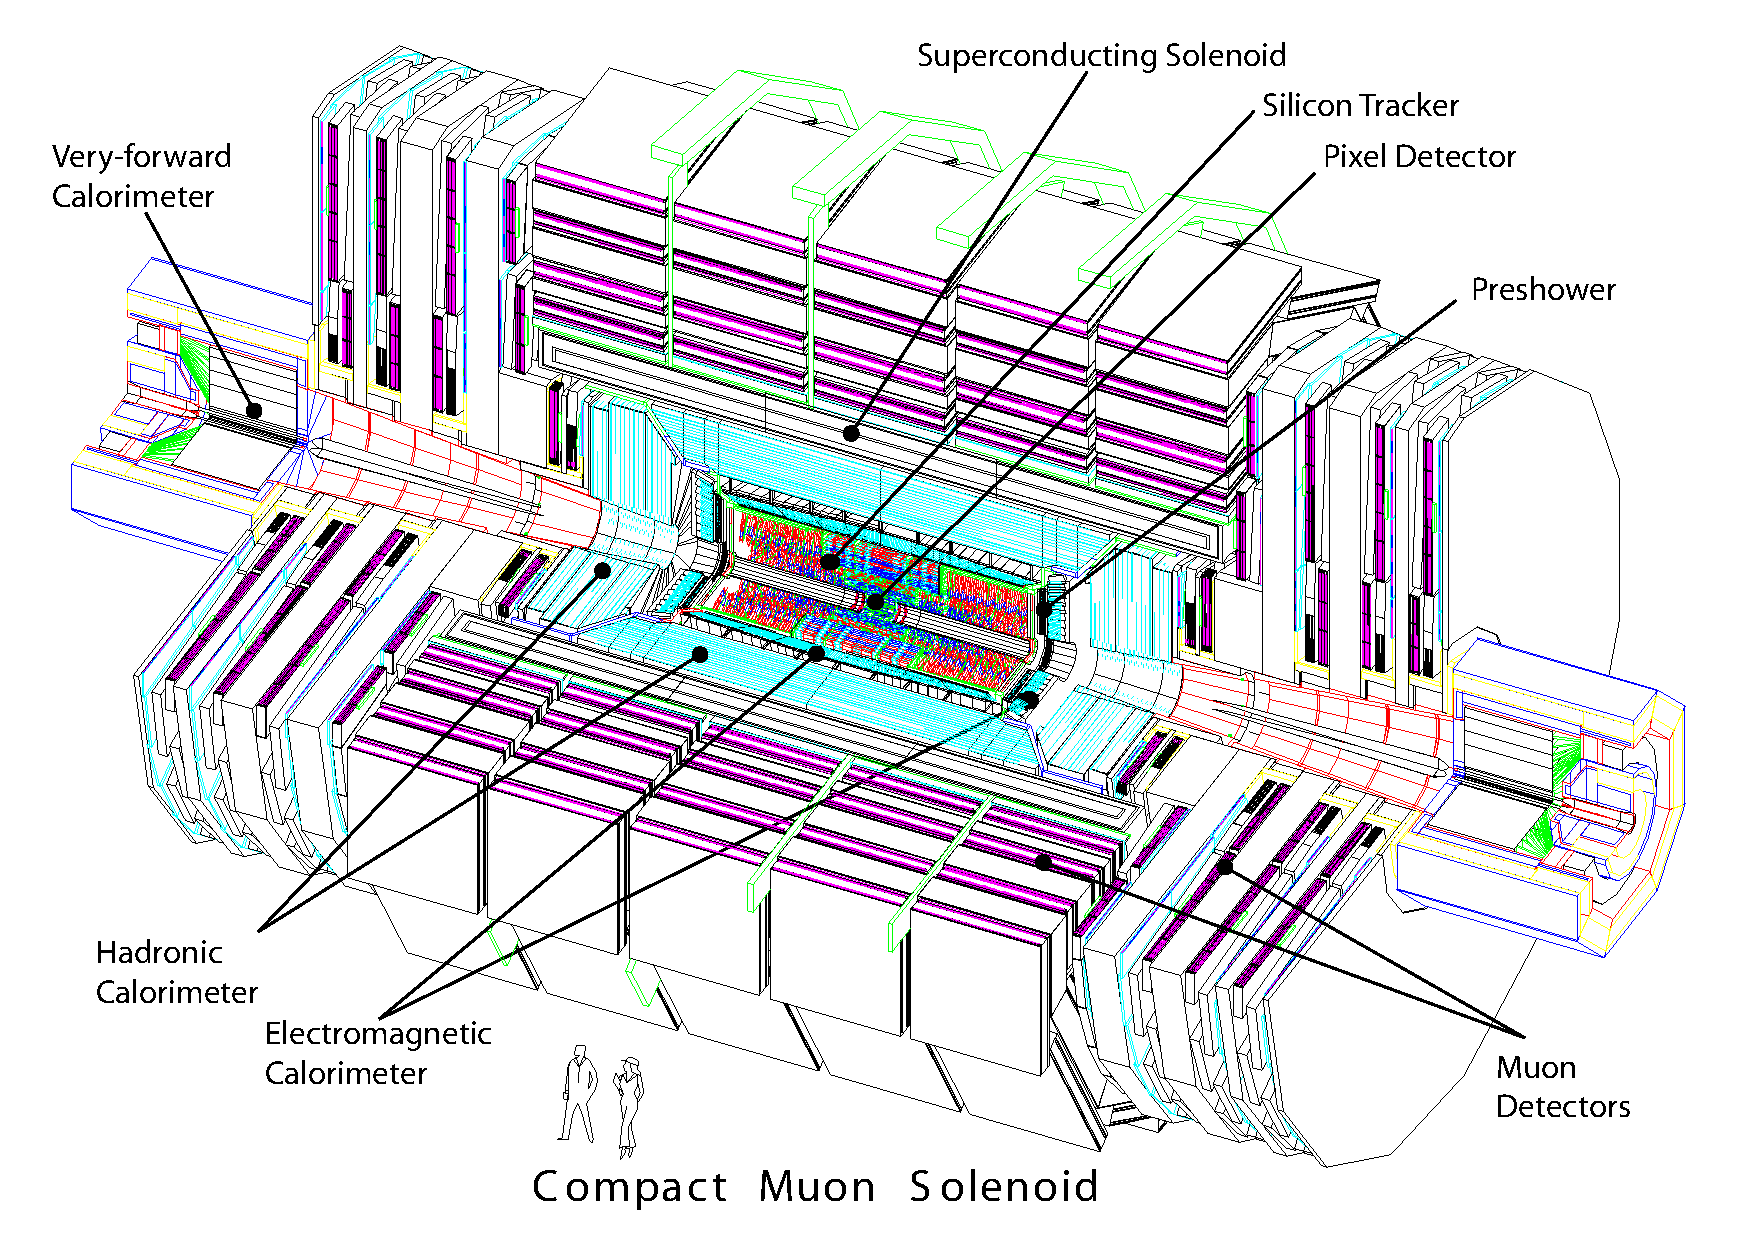
\includegraphics[width=0.1\textwidth]{Images/CMS_Layout.pdf}
\caption{Global track reconstruction efficiency for muons of several transverse momentum: 1, 10, 100 GeV.}
\label{Tracker_performance}
\end{figure}

\subsubsection{The pixel detector}
The pixel system is the part of the tracking system that is closest to the interaction region and covers a pseudorapidity range $-2.5 < \eta  < 2.5$, matching the acceptance of the central tracker. \figurename~\ref{Pixel_structure} shows the geometric pixel strcture as a function of pseudorapidity $\eta$. It contributes precise tracking points in $r - \phi$ and z and therefore is responsible for a small impact parameter resolution that is important for good secondary vertex reconstruction. With a pixel cell size of $100 \times 150\ \mu m^{2}$ emphasis has been put on achieving similar track resolution in both $r-\phi$ and z directions: 10 $\mu m$ in $r - \phi$ direction and 20 $\mu m$ along z. The pixel detector is essential for the reconstruction of secondary vertices from b and tau decays, and forming seed tracks for the outer track reconstruction and high level triggering. It consists of three barrel layers (BPix) with two endcap disks (FPix). The 53-cm-long BPix layers will be located at mean radii of 4.4, 7.3 and 10.2 cm. The FPix disks extending from $\approx$ 6 to 15 cm in radius, will be placed on each side at z=$\pm$34.5 and z=$\pm$46.5 cm. BPix (FPix) contain 48 million (18 million) pixels covering a total area of 0.78 (0.28) $m^{2}$. The arrangement of the 3 barrel layers and the forward pixel disks on each side gives 3 tracking points over almost the full $\eta$ range. In the high $\eta$ region the 2 disk points are combined with the lowest possible radius point from the 4.4 cm barrel layer.
\begin{figure}[htbp]
\centering
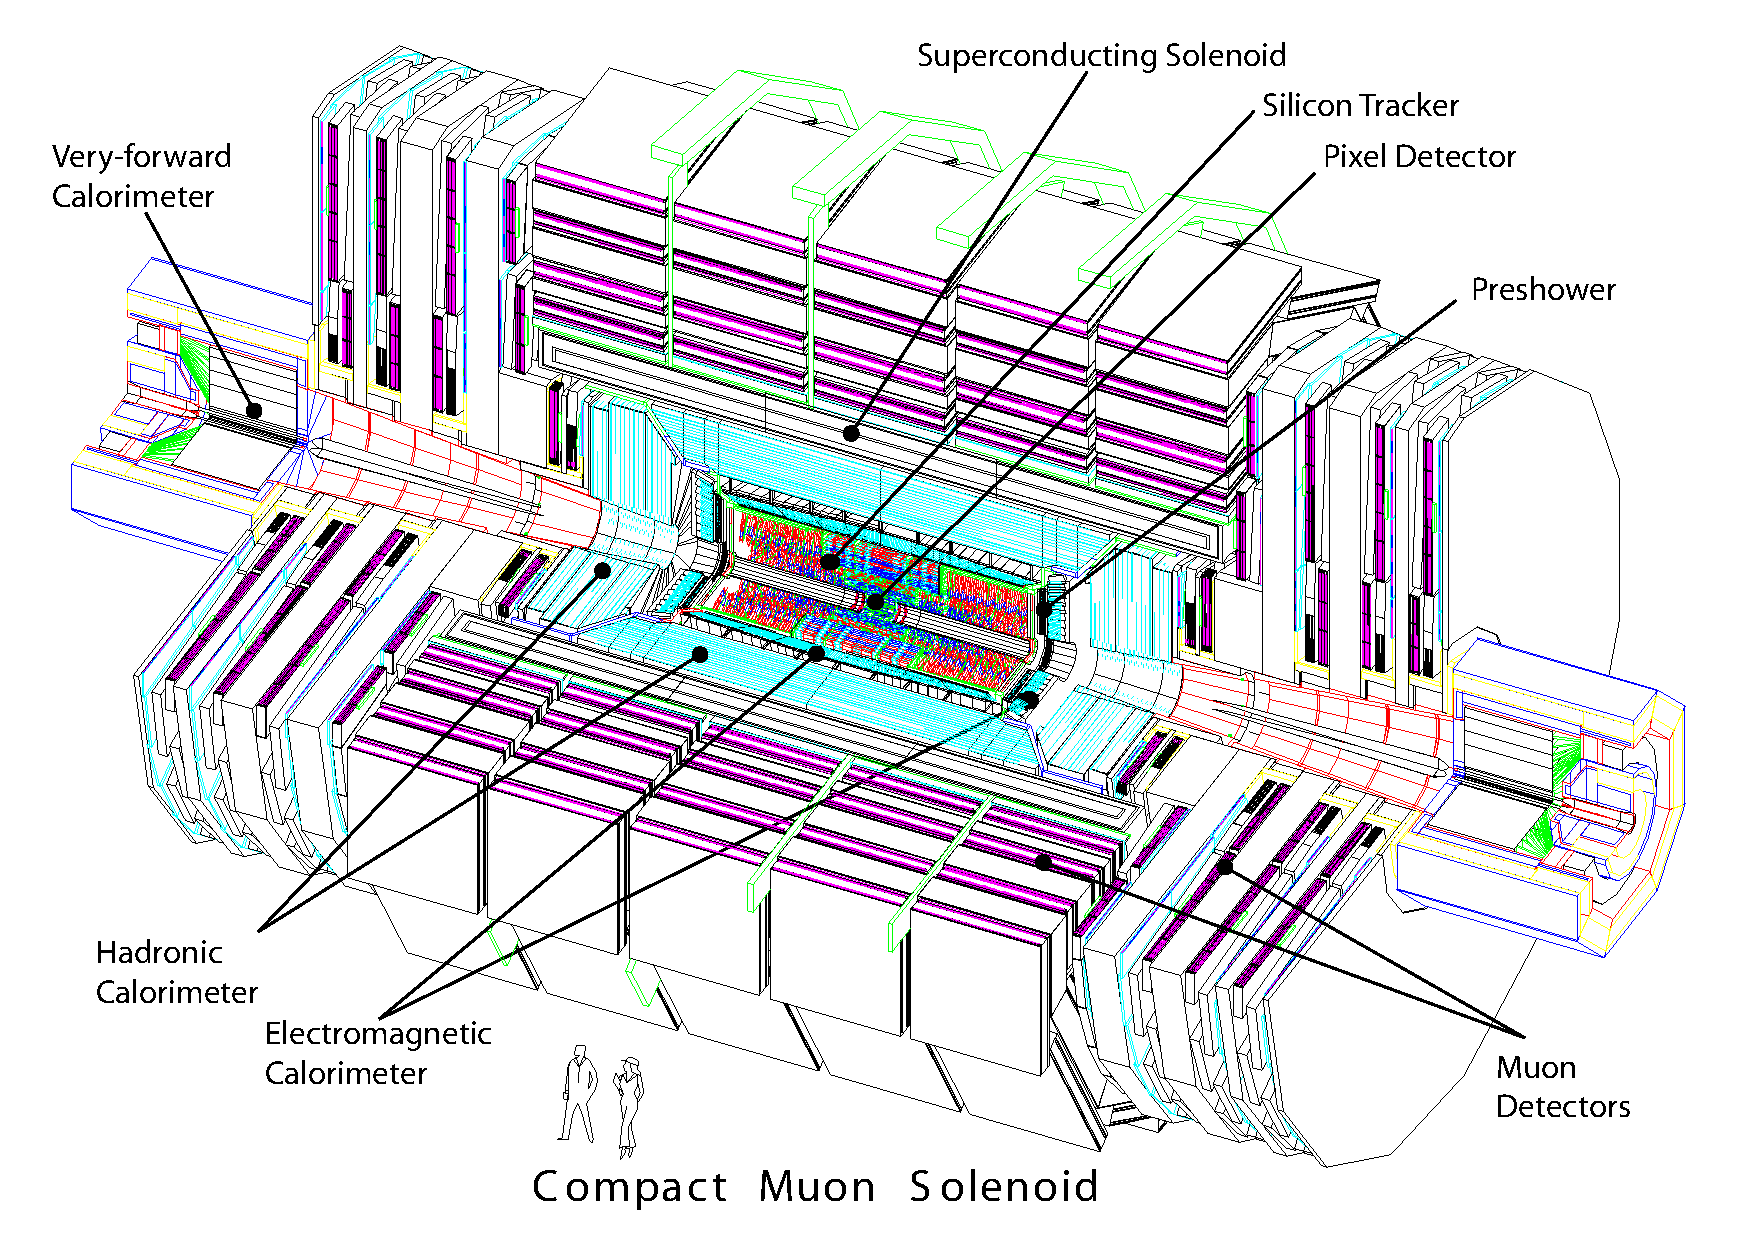
\includegraphics[width=0.1\textwidth]{Images/CMS_Layout.pdf}
\caption{Geometrical layout of the pixel detector as a function of pseudorapidity $\eta$.}
\label{Pixel_structure}
\end{figure}


\subsubsection{The silicon strip detector}
The silicon strip detector is composed of three different subsystem. The Tracker Inner Barrel and Disks (TIB/TID  see \figurename~\ref{tracking_system}) are composed of 4 barrel layers, supplemented by 3 disks at each end. TIB/TID delivers up to 4 $r-\phi$ measurements on a trajectory using 320 $\mu m$ thick silicon microstrip sensors with their strips parallel to the beam axis in the barrel and radial on the disks. The strip pitch is 80$\mu m$ on layers 1 and 2 and 120 $\mu m$ on layers 3 and 4 in the TIB, leading to a single point resolution of 23 $\mu m$ and 35 $\mu m$, respectively. In the TID the mean pitch varies between 100$\mu m$ and 141$\mu m$. The TIB/TID is surrounded by the Tracker Outer Barrel (TOB). It has an outer radius of 116 cm and consists of 6 barrel layers of 500$\mu m$ thick microstrip sensors with strip pitches of 183$\mu m$ on the first 4 layers and 122$\mu m$ on layers 5 and 6. It provides another 6 $r-\phi$ measurements with single point resolution of 53$\mu m$ and 35$\mu m$, respectively. The TOB extends in z between $\pm$118cm. Beyond this z range the Tracker EndCaps ($\pm$TEC, where the sign indicates the location along the z axis) cover the region 124 cm < |z| < 282 cm and 22.5 cm < |r| < 113.5 cm. Each TEC is composed of 9 disks, carrying up to 7 rings of silicon microstrip detectors (320$\mu m$ thick on the inner 4 rings, 500$\mu m$ thick on rings 5-7) with radial strips of 97$\mu m$ to 184$\mu m$ average pitch. Thus, they provide up to 9 $\phi$ measurements per trajectory. In addition, the modules in the first two layers and rings, respectively, of TIB, TID, and TOB as well as rings 1, 2, and 5 of the TECs carry a second microstrip detector module which is mounted back-to-back with a stereo angle of 100 mrad in order to provide a measurement of the second coordinate (z in the barrel and r on the disks). The achieved single point resolution of this measurement is 230$\mu m$ and 530$\mu m$ in TIB and TOB, respectively, and varies with pitch in TID and TEC. \\
The sensor elements in the strip tracker are single sided p-on-n type silicon micro-strip sensors shown in \figurename~\ref{Silicon_structure}: in TIB/TID and on the inner 4 rings of the TECs, thin sensors of (320 $\pm$ 20) $\mu m$ wafer thickness are used, with substrate resistivity of $ro$ = 1.55 - 3.25 k$\Omega$cm; TOB and the outer 3 rings of the TECs are equipped with thicker sensors of (500 $\pm$ 20) $\mu m$ thickness, with substrate resistivity of $ro$ = 4 - 8 k$\Omega$cm.
\begin{figure}[htbp]
\centering
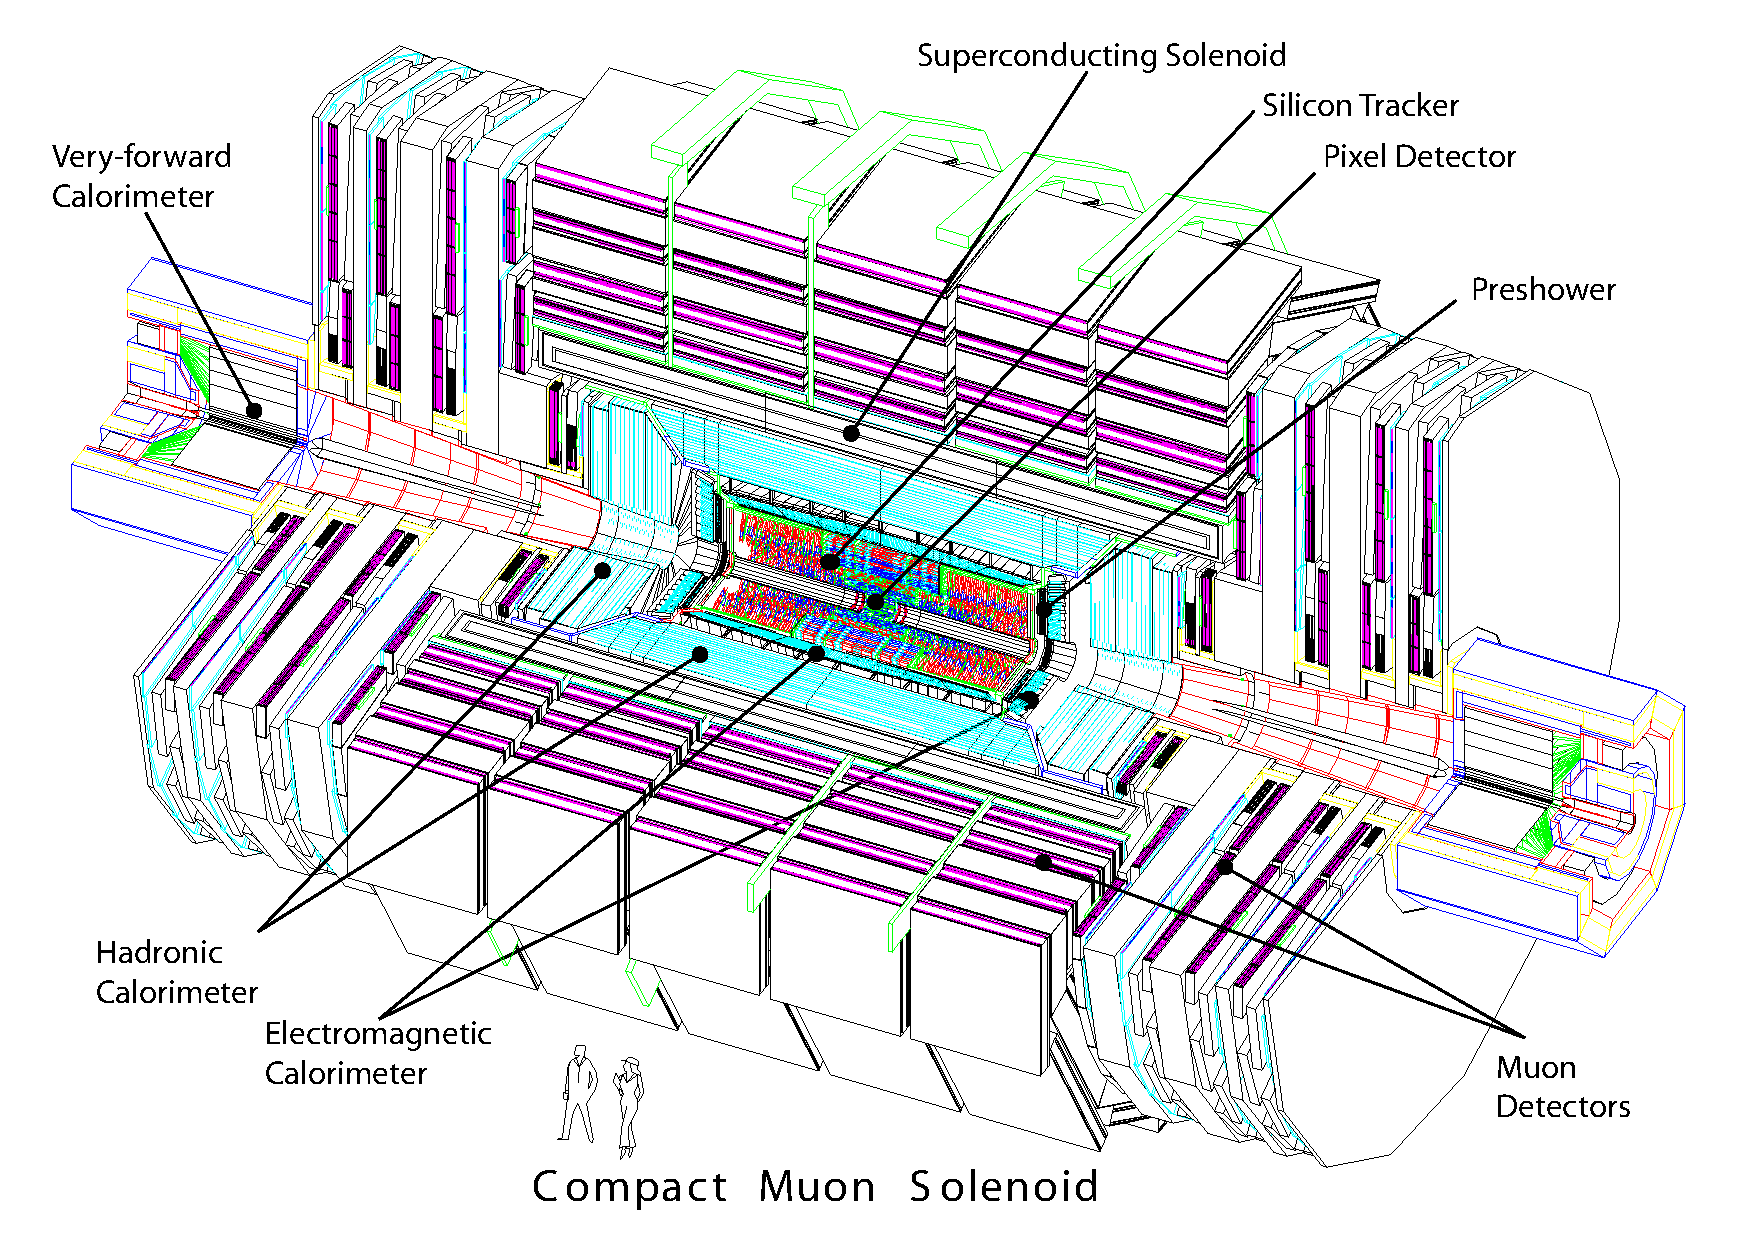
\includegraphics[width=0.1\textwidth]{Images/CMS_Layout.pdf}
\caption{Single sided p-on-n type silicon micro-strip sensor.}
\label{Silicon_structure}
\end{figure}
\\ LASER ALIGNMENT SYSTEM
\\ UPGRADE IN 2017
\subsection{Electromagnetic calorimeter}
The electromagnetic calorimeter of CMS (ECAL) is a hermetic homogeneous calorimeter made of 61200 lead tungstate ($PbWO_{4}$) crystals mounted in the central barrel part, closed by 7324 crystals in each of the two endcaps. A preshower detector is placed in front of the endcap crystals. Avalanche photodiodes (APDs) are used as photodetectors in the barrel and vacuum phototriodes (VPTs) in the endcaps. The use of high density crystals has allowed the design of a calorimeter which is fast, has fine granularity and is radiation resistant. One of the driving criteria in the design was the capability to detect the decay to two photons of the postulated Higgs boson. \\
The characteristics \cite{PbWO4}  of the $PbWO_{4}$ crystals make them an appropriate choice for operation at LHC. The high density (8.28$g/cm^{3}$), short radiation length (0.89 cm) and small Moli�re radius (2.2 cm) result in a fine granularity and a compact calorimeter. The scintillation decay time of these crystals is of the same order of magnitude as the LHC bunch crossing time: about 80\% of the light is emitted in 25 ns. The light output is relatively low and varies with temperature: at 18$^\circ$C about 4.5 photoelectrons per MeV are collected in both APDs and VPTs. The crystals emit blue-green scintillation light with a broad maximum at 420?430 nm. \\
The barrel part of the ECAL (EB) covers the pseudorapidity range $|\eta|$ < 1.479. The barrel granularity is 360 fold in $\phi$ and (2x85) fold in $\eta$, resulting in a total of 61200 crystals. The crystals have a tapered shape, slightly varying with position in $\eta$. They are mounted in a quasi-projective geometry to avoid cracks aligned with particle trajectories, so that their axes make a small angle ($3^\circ$) with respect to the vector from the nominal interaction vertex, in both the $\phi$ and $\eta$ projections. The crystal cross-section corresponds to approximately 0.0174x0.0174 in $\eta-\phi$ or 22x22 $mm^{2}$ at the front face of crystal, and 26x26 $mm^{2}$ at the rear face. The crystal length is 230 mm corresponding to 25.8 $X_{0}$ (where the symbol  $X_{0}$ stands for a \textit{radiation length}). The barrel crystal volume is 8.14 $m^{3}$ and the weight is 67.4 t. The endcaps (EE) cover the rapidity range 1.479 < $|\eta|$ < 3.0. The longitudinal distance between the interaction point and the endcap envelope is 315.4 cm, taking account of the estimated shift toward the interaction point by 1.6 cm when the 4-T magnetic field is switched on. The endcap consists of identically shaped crystals grouped in mechanical units of 5x5 crystals (supercrystals, or SCs) consisting of a carbon-fibre alveola structure. Each endcap is divided into 2 halves, or Dees. Each Dee holds 3662 crystals. These are contained in 138 standard SCs and 18 special partial supercrystals on the inner and outer circumference. The crystals and SCs are arranged in a rectangular x-y grid, with the crystals pointing at a focus 1300 mm beyond the interaction point, giving off-pointing angles ranging from 2 to 8 degrees. The crystals have a rear face cross section 30x30 $mm^{2}$, a front face cross section 28.62x28.62 $mm^{2}$ and a length of 220 mm (24.7 $X_{0}$). The endcaps crystal volume is 2.90 $m^{3}$ and the weight is 24.0 t. The layout of the calorimeter is shown in \figurename~\ref{ECAL}. \\
\begin{figure}[htbp]
\centering
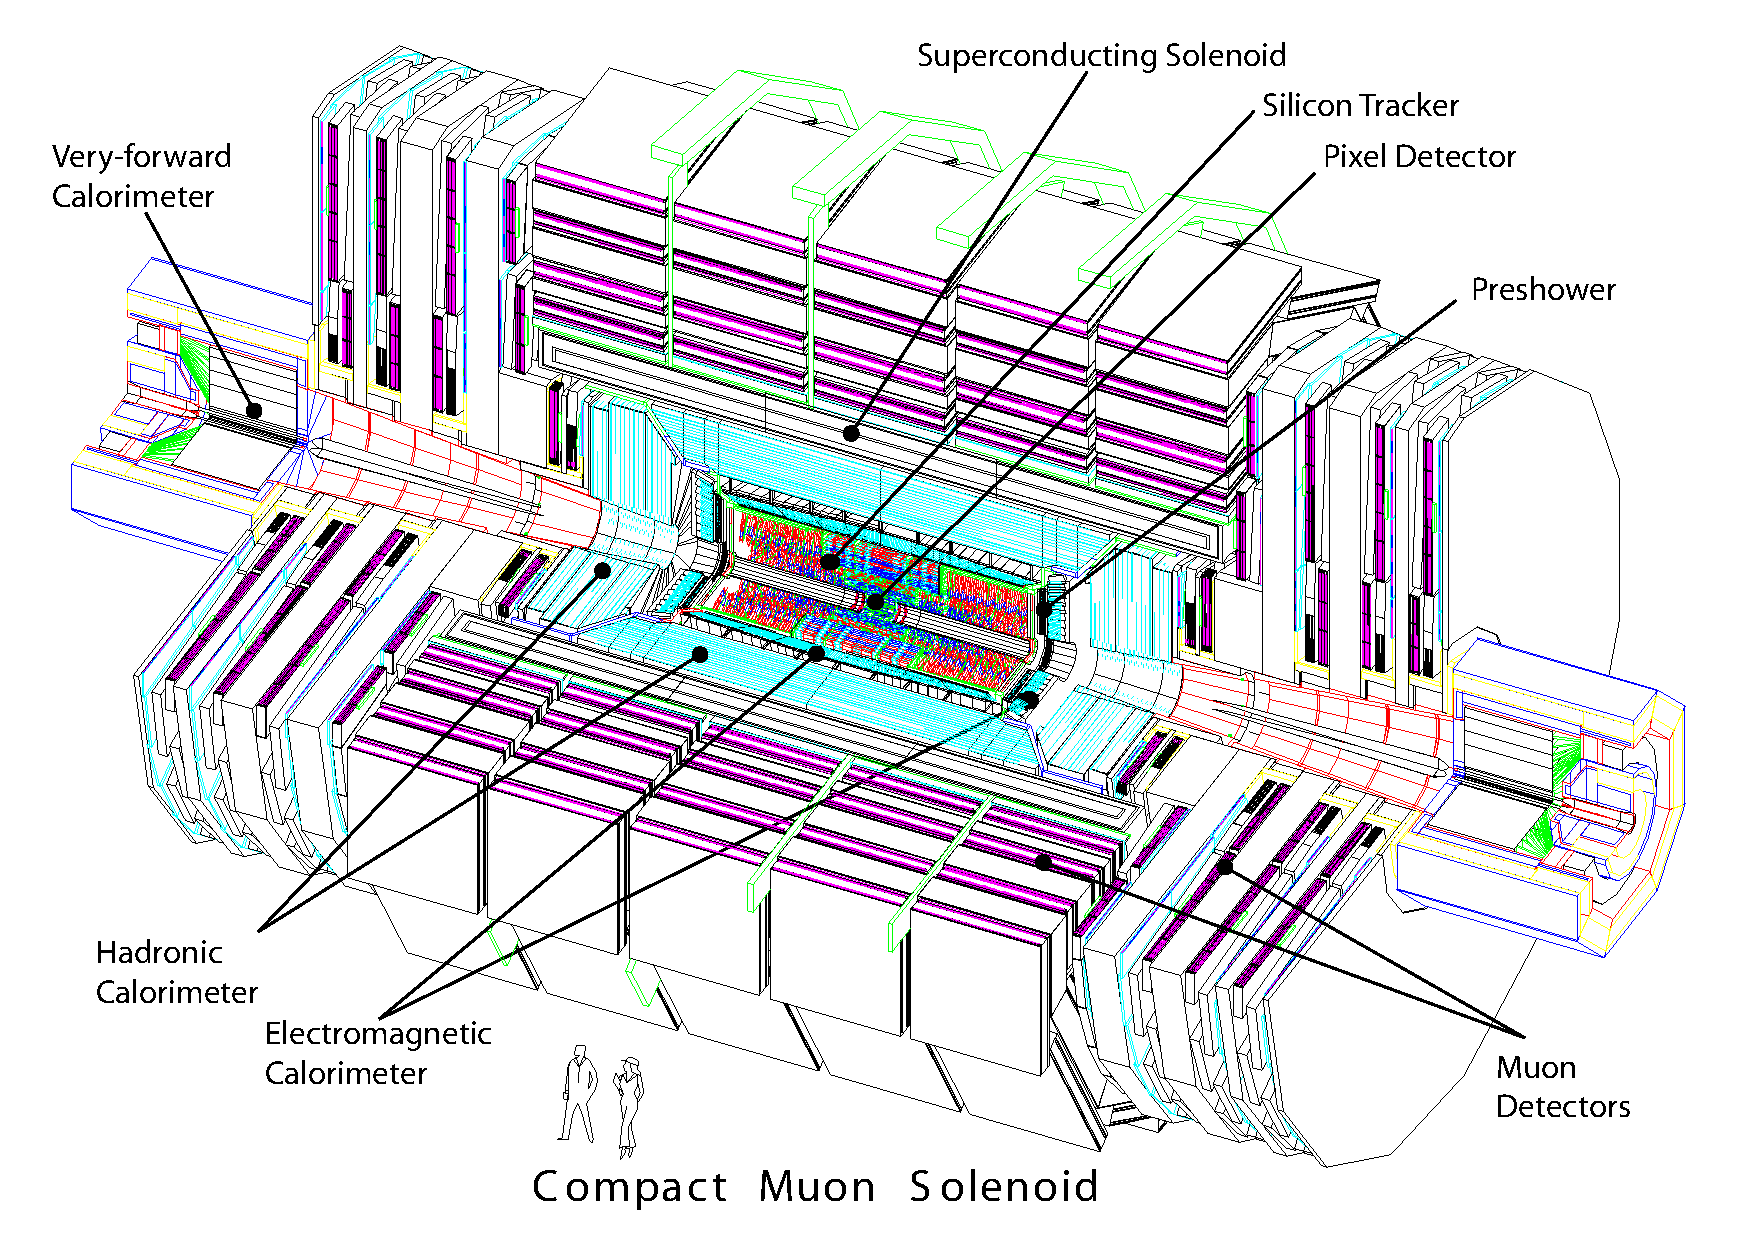
\includegraphics[width=0.1\textwidth]{Images/CMS_Layout.pdf}
\caption{Layout of the CMS electromagnetic calorimeter showing the arrangement of crystal modules, supermodules and endcaps, with the preshower in front.}
\label{ECAL}
\end{figure}

\subsubsection{Preshower detector}
The principal aim of the CMS Preshower detector is to identify neutral pions in the endcaps within a fiducial region 1.653 < $|\eta|$ < 2.6. It also helps the identification of electrons against minimum ionizing particles, and improves the position determination of electrons and photons with high granularity. The Preshower is a sampling calorimeter with two layers: lead radiators initiate electromagnetic showers from incoming photons/electrons whilst silicon strip sensors placed after each radia- tor measure the deposited energy and the transverse shower profiles. The total thickness of the Preshower is 20 cm. The material thickness of the Preshower traversed at $\eta$ = 1.653 before reaching the first sensor plane is 2 $X_{0}$, followed by a further 1 $X_{0}$ before reaching the second plane. Thus about 95\% of single incident photons start showering before the second sensor plane. The orientation of the strips in the two planes is orthogonal. 

\subsubsection{Energy resolution}
For energies below about 500 GeV, where shower leakage from the rear of the calorimeter starts to become significant, the energy resolution can be parametrized a:
\begin{equation}
\left(\frac{\sigma}{E}\right)^{2} = \left(\frac{S}{\sqrt{E}}\right)^2 + \left(\frac{N}{E}\right)^2  +C^{2}
\label{ECAL_resolution}
\end{equation}
where S is the stochastic term, N the noise term, and C the constant term. \\
The stochastic term has three basic contributions:
\begin{enumerate}
\item event-to-event fluctuations in the lateral shower containmen
\item a photostatistics contribution of 2.1\%
\item fluctuations in the energy deposited in the preshower absorber (where present) with respect to what is measured in the preshower silicon detector
\end{enumerate}
The contribution to the energy resolution from the preshower device can be approximately parametrized as a stochastic term with a value of 5\%/$\sqrt{E}$, where E is in GeV. But, because it samples only the beginning of the shower, the resolution is, in fact, predicted to vary like $\sigma$/E $\propto$ 1/$E^{0.75}$. \\
For the constant term instead, the main contributions are:
\begin{enumerate}
\item non-uniformity of the longitudinal light collection
\item intercalibration errors
\item leakage of energy from the back of the crystal
\end{enumerate}









